\chapter{量子力学与谐振子：阶梯算符}
\label{chap:e04}

\begin{chapteropening}
到目前为止，我们一直在说“光子”，却从没认真问过：光子究竟是从哪里冒出来的？它不是一颗事先就藏在真空里的小球，而是某个振动模式的一次“跳级”。要把这句话讲清楚，必须先回到量子力学里最朴素、也最重要的一个系统——谐振子（harmonic oscillator）。

本章的核心问题只有一个：一个来回振动的系统，它的能量为什么只能一格一格地取值？答案藏在两个算符里——一个专门“往下走一格”，一个专门“往上走一格”。它们叫做阶梯算符（ladder operators）。我们会从最普通的位置、动量出发，一步不跳地把这两个算符造出来，证明它们满足一条极其干净的对易关系，再用它们把能量谱、数态、零点能全部一次性读出来。这是整本书里“光子从哪来”的第一块基石：把这一章的代数吃透，后面所有关于相干态、热态、光子统计的讨论都只是它的推广。
\end{chapteropening}

\section{量子力学最小复习}
\label{sec:e04-review}

在动手之前，我们先把后面要反复用到的几件量子力学“工具”摆到桌面上。这一节不做证明，只是把你大概率见过一次的东西重新点亮一下；如果每一条你都觉得眼熟，那正说明你已经准备好了。

\paragraph{态矢量。}
一个量子系统在某一时刻的状态，用一个矢量 \(|\psi\rangle\) 表示，读作“ket psi”。你可以把它想成一支住在抽象空间（希尔伯特空间，Hilbert space）里的箭头。它的对偶伙伴写成 \(\langle\psi|\)（“bra psi”），两者拼起来 \(\langle\psi|\psi\rangle\) 就是这支箭头长度的平方。物理上我们总要求态是归一的：
\[
  \langle\psi|\psi\rangle=1,
\]
因为“系统一定处在某个状态”的总概率必须是 1。

\paragraph{算符与本征值。}
对系统能做的每一个物理测量（能量、位置、动量……），都对应一个算符（operator），我们用带帽子的字母表示，例如 \(\hat H,\hat x,\hat p\)。算符作用在态上会给出一个新态。特别地，如果某个态满足
\[
  \hat A\,|a\rangle = a\,|a\rangle,
\]
就说 \(|a\rangle\) 是 \(\hat A\) 的本征态（eigenstate），数 \(a\) 是对应的本征值（eigenvalue）。物理上，只有当系统正好处在 \(|a\rangle\) 时，测量 \(A\) 才会确定地得到 \(a\)。可观测量对应的算符都是厄米的（Hermitian，\(\hat A^\dagger=\hat A\)），这保证本征值是实数——测出来的数当然得是实的。

\paragraph{期望值。}
如果态不是本征态，测量结果就有涨落，我们只能谈平均值。在态 \(|\psi\rangle\) 上测量 \(A\)，多次重复的平均记为期望值（expectation value）
\begin{equation}
  \langle A\rangle \equiv \langle\psi|\,\hat A\,|\psi\rangle .
  \label{eq:e04-expectation}
\end{equation}
\begin{formulaexplain}
\(\langle A\rangle\) 是可观测量 \(A\) 在态 \(|\psi\rangle\) 上的平均测量值。把算符 \(\hat A\) 夹在 \(\langle\psi|\) 和 \(|\psi\rangle\) 中间即可。态若归一，它就是真正意义上的平均。
\end{formulaexplain}
这里 \(\hat A\) 是待测量对应的算符，\(|\psi\rangle\) 是系统当前的（归一）态。式 \eqref{eq:e04-expectation} 是我们本章反复要用的“提取数值”的唯一手段：一旦知道了态和算符，任何平均量都用它算出来。它没有单位问题——单位完全由 \(\hat A\) 决定，例如 \(\hat A=\hat H\) 时 \(\langle H\rangle\) 是能量（erg）。

\paragraph{对易子。}
两个算符先后作用的顺序一般不能交换，这种“不可交换”正是量子力学与经典力学的根本分野。我们用对易子（commutator）来度量它：
\begin{equation}
  [\hat A,\hat B]\equiv \hat A\hat B-\hat B\hat A .
  \label{eq:e04-commutator}
\end{equation}
\begin{formulaexplain}
\([\hat A,\hat B]\) 衡量“先 \(B\) 后 \(A\)”与“先 \(A\) 后 \(B\)”的差别。若它为零，两个量可以同时被精确测量；若不为零，它们互相“打架”。
\end{formulaexplain}
\(\hat A\hat B\) 表示先让 \(\hat B\) 作用、再让 \(\hat A\) 作用（算符从右往左作用在态上）。若 \([\hat A,\hat B]=0\)，我们说两算符对易，它们有共同的本征态，可以同时有确定值；若不为零，就不能。后面我们造阶梯算符时，几乎每一步化简都是在反复搬动这个 \(\hat A\hat B-\hat B\hat A\)。一条马上要用到的恒等式（直接展开即可验证）是
\[
  [\hat A,\hat B\hat C]=[\hat A,\hat B]\hat C+\hat B[\hat A,\hat C].
\]

\paragraph{正则对易关系。}
在所有对易子里，最基本的一条是位置和动量之间的正则对易关系（canonical commutation relation）：
\begin{equation}
  [\hat x,\hat p]=i\hbar .
  \label{eq:e04-xp}
\end{equation}
\begin{formulaexplain}
\(\hat x\) 是位置算符，\(\hat p\) 是动量算符，\(\hbar\) 是约化普朗克常数。它们不对易，差出一个纯虚常数 \(i\hbar\)。这是整个量子力学的“地基砖”。
\end{formulaexplain}
式 \eqref{eq:e04-xp} 里，\(\hat x\) 的量纲是长度（cm），\(\hat p\) 的量纲是动量（\(\mathrm{g\,cm\,s^{-1}}\)），乘积的量纲是作用量（\(\mathrm{erg\,s}\)），正好与 \(\hbar\) 一致（\(\hbar\simeq1.05\times10^{-27}\,\mathrm{erg\,s}\)）。注意右边是一个纯数乘以单位算符，与态无关——这正是它“基本”的原因。本章后面所有代数，归根到底只用到这一条 \([\hat x,\hat p]=i\hbar\)，其余全是逻辑推演。

\paragraph{测不准关系。}
两个不对易的量不能同时被无限精确地确定，这就是测不准关系（uncertainty relation）。它的一般形式叫罗伯逊不等式（Robertson inequality）：对任意两个厄米算符 \(\hat A,\hat B\)，在任意态上它们的标准差满足
\[
  \Delta A\,\Delta B\ \ge\ \frac12\big|\langle[\hat A,\hat B]\rangle\big| .
\]
这条不等式的右边正是由对易子决定的——两个量越“不对易”，就越无法同时确定。我们不在复习节里证明它，只把它作为已知结果拿来用。现在取 \(\hat A=\hat x,\hat B=\hat p\)，代入正则对易关系 \eqref{eq:e04-xp} 的 \([\hat x,\hat p]=i\hbar\)，右边的期望值 \(\langle i\hbar\rangle=i\hbar\)（它是个纯常数，与态无关），于是 \(\tfrac12|\langle[\hat x,\hat p]\rangle|=\tfrac12|i\hbar|=\hbar/2\)，得到最著名的一条：
\[
  \Delta x\,\Delta p\ \ge\ \frac{\hbar}{2},
\]
其中 \(\Delta x=\sqrt{\langle \hat x^2\rangle-\langle\hat x\rangle^2}\) 是位置的标准差，\(\Delta p\) 类似。它告诉我们：一个量子态不可能同时把位置和动量都压到零涨落。记住这个“最小面积 \(\hbar/2\)”，因为谐振子的基态恰好是把这个不等式取到等号的态——它是量子涨落所能达到的最“安静”的振动。这一节到此为止；我们已经把工具备齐了。

\section{量子谐振子与阶梯算符的构造}
\label{sec:e04-ladder}

现在进入正题。想象一颗小球拴在弹簧上来回振动，或者一个双原子分子里两个原子相对伸缩，或者——这才是我们真正关心的——电磁场里一个单一模式的振荡。它们在数学上是同一个系统：谐振子。在量子力学里，它的哈密顿量（Hamiltonian，即能量算符）是
\begin{equation}
  \hat H=\frac{\hat p^2}{2m}+\frac{1}{2}m\omega^2\hat x^2 .
  \label{eq:e04-hamiltonian}
\end{equation}
\begin{formulaexplain}
第一项 \(\hat p^2/2m\) 是动能，第二项 \(\tfrac12 m\omega^2\hat x^2\) 是弹簧势能。\(m\) 是质量，\(\omega\) 是振动角频率。整条式子就是“动能加势能”的量子版本。
\end{formulaexplain}
式 \eqref{eq:e04-hamiltonian} 里 \(m\) 是质量（g），\(\omega\) 是角频率（\(\mathrm{rad\,s^{-1}}\)），\(\hat x,\hat p\) 是上一节的位置、动量算符。整体量纲是能量（erg）。经典地，这个系统会以频率 \(\omega\) 做正弦振动，能量可以连续取任意正值。量子的问题是：\(\hat H\) 的本征值——也就是允许的能量——长什么样？

直接去解微分方程当然可以，但那样会淹没在特殊函数里。有一条优雅得多的路：把 \(\hat H\) 因式分解。注意 \(\hat p^2/2m+\tfrac12 m\omega^2\hat x^2\) 形状像 \(a^2+b^2\)，而 \(a^2+b^2=(a-ib)(a+ib)\)——只不过 \(\hat x\) 与 \(\hat p\) 不对易，因式分解会留下“尾巴”，那条尾巴恰恰藏着全部物理。为此我们定义两个新算符：
\begin{equation}
  \hat a=\sqrt{\frac{m\omega}{2\hbar}}\left(\hat x+\frac{i\,\hat p}{m\omega}\right),
  \qquad
  \hat a^\dagger=\sqrt{\frac{m\omega}{2\hbar}}\left(\hat x-\frac{i\,\hat p}{m\omega}\right).
  \label{eq:e04-adef}
\end{equation}
\begin{formulaexplain}
\(\hat a\) 是湮灭算符，\(\hat a^\dagger\) 是产生算符，二者互为厄米共轭。它们把有量纲的 \(\hat x,\hat p\) 打包成无量纲的组合，是通向能级阶梯的“钥匙”。
\end{formulaexplain}
先说量纲，确认这两个定义是“干净”的。系数 \(\sqrt{m\omega/2\hbar}\) 的量纲是 \(\sqrt{\mathrm{g}\cdot\mathrm{s^{-1}}/\mathrm{erg\,s}}=\mathrm{cm^{-1}}\)（因为 \(\mathrm{erg}=\mathrm{g\,cm^2\,s^{-2}}\)），乘上量纲为 cm 的 \(\hat x\)，得到一个纯数；而 \(\hat p/(m\omega)\) 的量纲是 \(\mathrm{g\,cm\,s^{-1}}/(\mathrm{g\,s^{-1}})=\mathrm{cm}\)，也乘成纯数。所以 \(\hat a,\hat a^\dagger\) 都是无量纲算符——这很重要，它们数的是“第几格”，本来就不该带单位。因为 \(\hat x,\hat p\) 是厄米算符，把式 \eqref{eq:e04-adef} 取厄米共轭（\(i\to -i\)）立刻看出 \(\hat a\) 与 \(\hat a^\dagger\) 确实互为共轭。

\paragraph{反解出 \(\hat x,\hat p\)。}
定义之后，我们常常需要反过来把 \(\hat x,\hat p\) 用 \(\hat a,\hat a^\dagger\) 表示。把式 \eqref{eq:e04-adef} 两式相加、相减即可：相加时虚部相消，相减时实部相消，
\[
  \hat a+\hat a^\dagger=\sqrt{\frac{m\omega}{2\hbar}}\,(2\hat x),
  \qquad
  \hat a-\hat a^\dagger=\sqrt{\frac{m\omega}{2\hbar}}\,\frac{2i\,\hat p}{m\omega}.
\]
于是
\begin{equation}
  \hat x=\sqrt{\frac{\hbar}{2m\omega}}\,(\hat a+\hat a^\dagger),
  \qquad
  \hat p=-i\sqrt{\frac{m\omega\hbar}{2}}\,(\hat a-\hat a^\dagger).
  \label{eq:e04-xp-in-a}
\end{equation}
\begin{formulaexplain}
把位置和动量重新写成产生、湮灭算符的组合。\(\hat x\) 对应“对称”组合 \(\hat a+\hat a^\dagger\)，\(\hat p\) 对应“反对称”组合 \(\hat a-\hat a^\dagger\)，各自配一个带量纲的前因子。
\end{formulaexplain}
这两条以后会反复用到：任何含 \(\hat x,\hat p\) 的量（比如电场，它正比于 \(\hat x\)）都能翻译成产生、湮灭算符的语言。前因子 \(\sqrt{\hbar/2m\omega}\) 的量纲正好是 cm，\(\sqrt{m\omega\hbar/2}\) 正好是动量单位，量纲自洽。

\paragraph{关键一步：算出 \([\hat a,\hat a^\dagger]\)。}
这是全章最重要的代数，我们一步不跳地做。把定义式 \eqref{eq:e04-adef} 代入对易子，先把常数系数 \(m\omega/2\hbar\) 提到前面：
\[
  [\hat a,\hat a^\dagger]
  =\frac{m\omega}{2\hbar}
  \left[\hat x+\frac{i\hat p}{m\omega},\ \hat x-\frac{i\hat p}{m\omega}\right].
\]
对易子对两边都是线性的，把它按四项展开：
\[
  \left[\hat x+\tfrac{i\hat p}{m\omega},\ \hat x-\tfrac{i\hat p}{m\omega}\right]
  =[\hat x,\hat x]
  -\frac{i}{m\omega}[\hat x,\hat p]
  +\frac{i}{m\omega}[\hat p,\hat x]
  -\frac{i^2}{(m\omega)^2}[\hat p,\hat p].
\]
现在逐项处理。任何算符和自己对易，所以 \([\hat x,\hat x]=[\hat p,\hat p]=0\)，第一项和第四项直接消失。中间两项用正则对易关系 \eqref{eq:e04-xp}：\([\hat x,\hat p]=i\hbar\)，而 \([\hat p,\hat x]=-[\hat x,\hat p]=-i\hbar\)。代入：
\[
  =-\frac{i}{m\omega}(i\hbar)+\frac{i}{m\omega}(-i\hbar)
  =-\frac{i^2\hbar}{m\omega}-\frac{i^2\hbar}{m\omega}
  =\frac{\hbar}{m\omega}+\frac{\hbar}{m\omega}
  =\frac{2\hbar}{m\omega},
\]
这里用了 \(i^2=-1\)。把它乘回前面的系数：
\[
  [\hat a,\hat a^\dagger]=\frac{m\omega}{2\hbar}\cdot\frac{2\hbar}{m\omega}=1.
\]
于是我们得到本章的“主定理”：
\begin{equation}
  [\hat a,\hat a^\dagger]=1 .
  \label{eq:e04-aacomm}
\end{equation}
\begin{formulaexplain}
产生与湮灭算符的对易子等于 1。这条极简的关系是谐振子（以及后面每一个光场模式）全部量子结构的源头，能级、光子、零点能都从它长出来。
\end{formulaexplain}
请体会这条式子有多干净：有量纲的 \(\hat x,\hat p\)、有单位的 \(m,\omega,\hbar\) 全部约掉，只剩一个赤裸裸的 1。它无量纲，与具体是哪种振子无关。式 \eqref{eq:e04-aacomm} 会成为我们唯一需要记住的对易关系——从这一刻起，我们几乎可以把 \(\hat x,\hat p\) 忘掉，只在 \(\hat a,\hat a^\dagger\) 的代数里工作。作为对比，产生算符之间、湮灭算符之间当然对易：\([\hat a,\hat a]=[\hat a^\dagger,\hat a^\dagger]=0\)。

\section{用数算符改写哈密顿量}
\label{sec:e04-numberH}

造出 \(\hat a,\hat a^\dagger\) 是为了简化 \(\hat H\)。现在我们把式 \eqref{eq:e04-hamiltonian} 翻译成产生、湮灭算符的语言。最省事的做法是先算组合 \(\hat a^\dagger\hat a\)，看看它离 \(\hat H\) 有多远。用定义 \eqref{eq:e04-adef}，把系数提出：
\[
  \hat a^\dagger\hat a
  =\frac{m\omega}{2\hbar}
  \left(\hat x-\frac{i\hat p}{m\omega}\right)\!\left(\hat x+\frac{i\hat p}{m\omega}\right).
\]
小心地把括号乘开（注意保持算符顺序，因为它们不对易）：
\[
  \left(\hat x-\tfrac{i\hat p}{m\omega}\right)\!\left(\hat x+\tfrac{i\hat p}{m\omega}\right)
  =\hat x^2+\frac{i}{m\omega}\hat x\hat p-\frac{i}{m\omega}\hat p\hat x-\frac{i^2}{(m\omega)^2}\hat p^2 .
\]
把中间两项合起来，它们正是一个对易子：\(\dfrac{i}{m\omega}(\hat x\hat p-\hat p\hat x)=\dfrac{i}{m\omega}[\hat x,\hat p]=\dfrac{i}{m\omega}(i\hbar)=-\dfrac{\hbar}{m\omega}\)。而最后一项 \(-i^2\hat p^2/(m\omega)^2=+\hat p^2/(m\omega)^2\)。于是
\[
  \hat a^\dagger\hat a
  =\frac{m\omega}{2\hbar}
  \left(\hat x^2+\frac{\hat p^2}{(m\omega)^2}-\frac{\hbar}{m\omega}\right)
  =\frac{m\omega}{2\hbar}\hat x^2+\frac{1}{2\hbar m\omega}\hat p^2-\frac12 .
\]
把前两项各乘一个 \(\hbar\omega\) 看它们是不是 \(\hat H\)：
\[
  \hbar\omega\left(\frac{m\omega}{2\hbar}\hat x^2\right)=\frac12 m\omega^2\hat x^2,
  \qquad
  \hbar\omega\left(\frac{1}{2\hbar m\omega}\hat p^2\right)=\frac{\hat p^2}{2m}.
\]
这正好是式 \eqref{eq:e04-hamiltonian} 的势能项和动能项！所以 \(\hbar\omega\,\hat a^\dagger\hat a=\hat H-\tfrac12\hbar\omega\)，整理即得
\begin{equation}
  \hat H=\hbar\omega\left(\hat a^\dagger\hat a+\frac12\right)
        =\hbar\omega\left(\hat n+\frac12\right),
  \qquad \hat n\equiv\hat a^\dagger\hat a .
  \label{eq:e04-Hn}
\end{equation}
\begin{formulaexplain}
哈密顿量被写成数算符 \(\hat n=\hat a^\dagger\hat a\) 的简单线性函数。能量等于“激发格数 \(\hat n\) 加上半格”再乘以 \(\hbar\omega\)。那半格就是零点能。
\end{formulaexplain}
这里 \(\hat n=\hat a^\dagger\hat a\) 叫数算符（number operator），它是厄米的（\((\hat a^\dagger\hat a)^\dagger=\hat a^\dagger\hat a\)），因此有实本征值——我们马上会看到它的本征值恰好是 \(0,1,2,\ldots\)，也就是“这个模式里有几个量子”。式 \eqref{eq:e04-Hn} 把求能谱的问题彻底简化：只要知道 \(\hat n\) 的本征值，能量就读出来了。量纲上，\(\hat n\) 无量纲，\(\hbar\omega\) 是能量，一切自洽。

\paragraph{零点能。}
式 \eqref{eq:e04-Hn} 里那个 \(+\tfrac12\) 不是可有可无的常数。即使 \(\hat n\) 取最小值 0，能量也不是零，而是
\[
  E_0=\frac12\hbar\omega .
\]
这就是零点能（zero-point energy）。物理上它是测不准关系的直接后果：如果振子真的静止在势阱底部，那它就同时有了确定的位置（\(x=0\)）和确定的动量（\(p=0\)），违反 \(\Delta x\,\Delta p\ge\hbar/2\)。量子力学不允许这种“绝对的安静”，于是即便在基态，振子也必须保有一份最低限度的抖动，对应能量 \(\tfrac12\hbar\omega\)。这份抖动不是我们测量能力的不足，而是真空本身的性质——后面讲光场时，正是这份“真空涨落”给出散粒噪声与压缩态的物理起点。给个数量级：可见光一个模式 \(\nu\sim6\times10^{14}\,\mathrm{Hz}\)，\(\hbar\omega=h\nu\simeq(6.6\times10^{-27})(6\times10^{14})\,\mathrm{erg}\simeq4\times10^{-12}\,\mathrm{erg}\approx2.5\,\mathrm{eV}\)，零点能约 1.2 eV——一个绝非可以忽略的量。

\section{数态：能量的一格一格}
\label{sec:e04-numberstates}

现在来读能谱。由式 \eqref{eq:e04-Hn}，\(\hat H\) 和 \(\hat n\) 只差一个常数和一个正因子，它们共享本征态。设 \(\hat n\) 的本征态为 \(|n\rangle\)，本征值为 \(n\)：
\[
  \hat n\,|n\rangle=n\,|n\rangle .
\]
我们把 \(|n\rangle\) 叫数态或福克态（number state / Fock state）。眼下 \(n\) 还只是一个待定的实数；这一节的任务，就是用对易关系 \eqref{eq:e04-aacomm} 逼出它只能是非负整数，并顺便求出 \(\hat a,\hat a^\dagger\) 作用在 \(|n\rangle\) 上到底给出什么。

\paragraph{阶梯算符为什么“爬楼梯”。}
先算两条关键的对易子。用 \([\hat a,\hat a^\dagger]=1\)：
\[
  [\hat n,\hat a]=[\hat a^\dagger\hat a,\hat a]
  =\hat a^\dagger[\hat a,\hat a]+[\hat a^\dagger,\hat a]\hat a
  =0+(-1)\hat a=-\hat a,
\]
其中用了展开恒等式 \([\hat A\hat B,\hat C]=\hat A[\hat B,\hat C]+[\hat A,\hat C]\hat B\) 以及 \([\hat a^\dagger,\hat a]=-1\)。同理
\[
  [\hat n,\hat a^\dagger]=\hat a^\dagger[\hat a,\hat a^\dagger]+[\hat a^\dagger,\hat a^\dagger]\hat a
  =\hat a^\dagger(1)+0=+\hat a^\dagger .
\]
这两条 \([\hat n,\hat a]=-\hat a\)、\([\hat n,\hat a^\dagger]=+\hat a^\dagger\) 就是“阶梯”的机械原理。看它们如何起作用：把 \(\hat n\) 作用在新态 \(\hat a|n\rangle\) 上，
\[
  \hat n\,(\hat a|n\rangle)
  =(\hat a\hat n+[\hat n,\hat a])|n\rangle
  =(\hat a\hat n-\hat a)|n\rangle
  =\hat a(\hat n-1)|n\rangle
  =(n-1)\,\hat a|n\rangle .
\]
读这行字：\(\hat a|n\rangle\) 又是 \(\hat n\) 的本征态，本征值降了 1，变成 \(n-1\)。所以 \(\hat a\) 把系统“往下带一格”，这就是它被叫做湮灭算符（annihilation operator）的原因。完全对称地，
\[
  \hat n\,(\hat a^\dagger|n\rangle)=(n+1)\,\hat a^\dagger|n\rangle,
\]
\(\hat a^\dagger\) 把系统“往上抬一格”，是产生算符（creation operator）。这就是“阶梯”二字的来历。

\paragraph{阶梯必须有底：\(n\) 是非负整数。}
为什么台阶不能无限往下延伸到负数？因为 \(\hat n\) 的本征值不可能为负。用式 \eqref{eq:e04-expectation}，对归一的 \(|n\rangle\) 算 \(\hat n\) 的期望值：
\[
  n=\langle n|\hat n|n\rangle=\langle n|\hat a^\dagger\hat a|n\rangle
  =\big(\hat a|n\rangle\big)^\dagger\big(\hat a|n\rangle\big)
  =\big\|\,\hat a|n\rangle\,\big\|^2\ \ge 0 .
\]
关键就在中间这步：\(\langle n|\hat a^\dagger\hat a|n\rangle\) 是态 \(\hat a|n\rangle\) 与自己的内积，也就是它长度的平方，而任何矢量长度的平方都非负。所以 \(n\ge0\)。可是 \(\hat a\) 每作用一次就把本征值减 1，若从某个非整数的 \(n\) 出发反复作用 \(\hat a\)，迟早会跌破 0，得到一个负本征值——矛盾。唯一的出路是：这串下降必须在某一步正好落到 0 然后停住，也就是存在一个基态 \(|0\rangle\) 满足
\begin{equation}
  \hat a\,|0\rangle=0 .
  \label{eq:e04-ground}
\end{equation}
\begin{formulaexplain}
湮灭算符作用在基态上给出零（不是态 \(|0\rangle\)，而是零矢量）。这表示“已经到最底层，再往下没有台阶了”。基态是整座能量阶梯的地板。
\end{formulaexplain}
只有当下降序列在 \(n=0\) 处被式 \eqref{eq:e04-ground} 掐断，才不会出现负本征值。由此倒推：从 \(|0\rangle\) 一步步用 \(\hat a^\dagger\) 往上爬，得到的本征值只能是 \(0,1,2,3,\ldots\)。换句话说，谐振子的激发数只能是非负整数——这正是“光子只能一个一个地有”的数学根源。

\paragraph{归一化系数：那两个 \(\sqrt{\ }\) 从哪来。}
我们已知 \(\hat a|n\rangle\) 正比于 \(|n-1\rangle\)，但比例常数是多少？这一步必须算全，因为后面光子统计里的因子全靠它。设 \(\hat a|n\rangle=c_n|n-1\rangle\)，其中 \(c_n\) 是待定常数，且 \(|n-1\rangle\) 已归一。两边取模平方：
\[
  \big\|\hat a|n\rangle\big\|^2
  =|c_n|^2\,\langle n-1|n-1\rangle
  =|c_n|^2 .
\]
而左边我们刚算过：\(\big\|\hat a|n\rangle\big\|^2=\langle n|\hat a^\dagger\hat a|n\rangle=\langle n|\hat n|n\rangle=n\)。所以 \(|c_n|^2=n\)，取正实的相位约定得 \(c_n=\sqrt{n}\)。完全类似地，为求 \(\hat a^\dagger|n\rangle=d_n|n+1\rangle\)，我们需要 \(\hat a\hat a^\dagger\) 的作用；由 \eqref{eq:e04-aacomm}，\(\hat a\hat a^\dagger=\hat a^\dagger\hat a+1=\hat n+1\)，于是
\[
  \big\|\hat a^\dagger|n\rangle\big\|^2
  =\langle n|\hat a\hat a^\dagger|n\rangle
  =\langle n|(\hat n+1)|n\rangle
  =n+1
  =|d_n|^2,
\]
给出 \(d_n=\sqrt{n+1}\)。把两条结论并排写出：
\begin{equation}
  \hat a\,|n\rangle=\sqrt{n}\,|n-1\rangle,
  \qquad
  \hat a^\dagger\,|n\rangle=\sqrt{n+1}\,|n+1\rangle .
  \label{eq:e04-ladder-action}
\end{equation}
\begin{formulaexplain}
湮灭算符把 \(|n\rangle\) 降到 \(|n-1\rangle\)，带系数 \(\sqrt{n}\)；产生算符把它升到 \(|n+1\rangle\)，带系数 \(\sqrt{n+1}\)。这两个平方根因子在后面所有光子计数公式里都会露面。
\end{formulaexplain}
注意两个细节。其一，当 \(n=0\) 时 \(\sqrt{n}=0\)，第一式自动退化成 \(\hat a|0\rangle=0\)，与式 \eqref{eq:e04-ground} 一致——地板确实封住了。其二，系数不是简单的 1，而是 \(\sqrt n\) 和 \(\sqrt{n+1}\)：正是这种“越高的台阶，跨步越大”的非线性，让相干态和热态的光子统计呈现出各自独特的形状。式 \eqref{eq:e04-ladder-action} 也给出构造任意数态的配方：反复用 \(\hat a^\dagger\) 从基态往上搭，
\[
  |n\rangle=\frac{(\hat a^\dagger)^n}{\sqrt{n!}}\,|0\rangle,
\]
其中 \(\sqrt{n!}\) 正是把一路上的 \(\sqrt{1}\cdot\sqrt{2}\cdots\sqrt{n}\) 累乘起来的结果。

\paragraph{能级：等间距的梯子。}
把 \(\hat n|n\rangle=n|n\rangle\) 代回式 \eqref{eq:e04-Hn}，能量本征值立刻读出：
\begin{equation}
  E_n=\hbar\omega\left(n+\frac12\right),\qquad n=0,1,2,\ldots
  \label{eq:e04-energy}
\end{equation}
\begin{formulaexplain}
第 \(n\) 个能级的能量。相邻能级间隔恒为 \(\hbar\omega\)，最低能级不是 0 而是 \(\tfrac12\hbar\omega\)。整座能谱是一把均匀的梯子，底座抬高了半格。
\end{formulaexplain}
式 \eqref{eq:e04-energy} 是本章的收获总账。它有两个鲜明特征。第一，能级是离散的、等间距的：相邻两级永远差 \(E_{n+1}-E_n=\hbar\omega\)，不多不少。正因为这份“恒定的一格”，我们才能干脆地说“吸收一个 \(\hbar\omega\) 的量子就上一层，放出一个就下一层”——这一个量子，对电磁场模式而言就是一个光子。落到真实数量级看看这“一格”有多大：一个典型双原子分子的伸缩振动 \(\omega/2\pi\sim10^{13}\text{--}10^{14}\,\mathrm{Hz}\)（红外波段），相邻能级间隔 \(\hbar\omega\sim0.1\text{--}0.5\,\mathrm{eV}\)，正好是红外光谱线的能量；而我们真正关心的可见光单模，\(\nu\sim6\times10^{14}\,\mathrm{Hz}\)，一格就是 \(\hbar\omega\approx2.5\,\mathrm{eV}\)，恰是一个可见光光子的能量。同一把梯子，换个 \(\omega\) 就从分子振动跨到光场。第二，底座被零点能抬到了 \(\tfrac12\hbar\omega\)，如上一节所述。把 \(E_n\) 画出来，就是一把从 \(\tfrac12\hbar\omega\) 起步、每级升高 \(\hbar\omega\) 的等距梯子；数态 \(|n\rangle\) 就是站在第 \(n\) 级上的态，携带 \(n\) 个能量量子。到这里，”光子从哪来”这个问题在单个模式上已经有了完整答案：光子就是谐振子能量阶梯上的一格激发，\(\hat a^\dagger\) 生出它，\(\hat a\) 湮灭它。图~\ref{fig:e04-energy-ladder} 把这把”梯子”整个画了出来。

\begin{figure}[tbp]
\centering
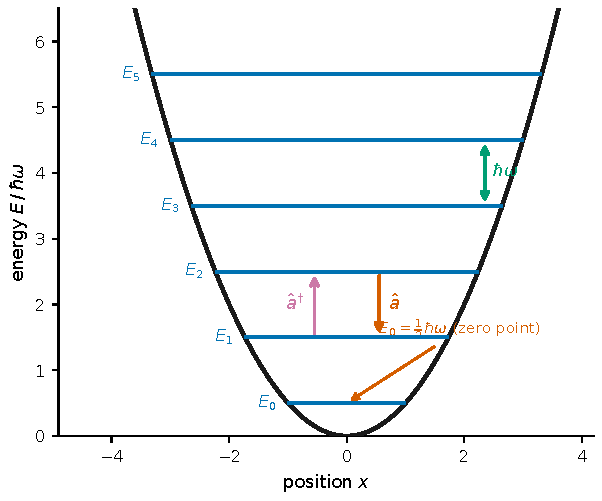
\includegraphics[width=0.6\linewidth]{figures/generated/edu_ch04/e04_energy_ladder.pdf}
\caption{量子谐振子的能量阶梯。在势阱 \(V(x)=\tfrac12 m\omega^2 x^2\) 里，允许的能量只能取等间距的一格一格 \(E_n=\hbar\omega(n+\tfrac12)\)：相邻两级永远相差 \(\hbar\omega\)（绿色双箭头），最低一级不是零，而是零点能 \(\tfrac12\hbar\omega\)（橙色）。产生算符 \(\hat a^\dagger\) 把系统抬高一格、湮灭算符 \(\hat a\) 压低一格。这”恒定的一格” \(\hbar\omega\)，对一个电磁场模式而言，就是一个光子的能量。}
\label{fig:e04-energy-ladder}
\end{figure}

\section{预告：最接近经典振动的量子态}
\label{sec:e04-coherent}

数态 \(|n\rangle\) 能量最确定，却也最“不像”经典振动。想想看：一个经典振子的位置随时间画出漂亮的正弦曲线 \(x(t)=x_0\cos\omega t\)，可数态的位置期望值 \(\langle n|\hat x|n\rangle\) 恒等于零——用式 \eqref{eq:e04-xp-in-a}，\(\hat x\propto\hat a+\hat a^\dagger\) 只会把 \(|n\rangle\) 变成 \(|n\pm1\rangle\)，与 \(\langle n|\) 正交，内积为零。也就是说，一个能量确定的量子振子，位置期望值根本不摆动，它在相空间里是一圈均匀模糊的环，完全没有“此刻在哪一侧”的信息。这与我们对“振动”的日常直觉正好相反。

那么，哪一种量子态才最像经典的来回摆动？答案是相干态（coherent state）\(|\alpha\rangle\)，它被定义为湮灭算符的本征态：
\begin{equation}
  \hat a\,|\alpha\rangle=\alpha\,|\alpha\rangle,\qquad \alpha\in\mathbb{C}.
  \label{eq:e04-coherent}
\end{equation}
\begin{formulaexplain}
相干态是湮灭算符 \(\hat a\) 的本征态，本征值 \(\alpha\) 是一个复数。复数的模给出平均光子数、幅角给出振动相位。它是“最接近经典”的量子态。
\end{formulaexplain}
这个定义初看很奇怪——\(\hat a\) 不是厄米算符，本征值 \(\alpha\) 允许是复数。但正是这个复数替我们同时编码了振幅和相位：\(|\alpha|\) 决定振动多强（可以证明平均光子数 \(\langle\hat n\rangle=|\alpha|^2\)），\(\arg\alpha\) 决定此刻摆到了哪个相位。可以证明，相干态的位置期望值确实随时间做正弦振动，而且它把位置与动量的联合涨落压到测不准关系允许的最小值——它是一团大小恒定、随时间沿圆周匀速平移的小“光斑”，看上去就像一个带着量子模糊的经典点。

不妨在脑子里把这两种态画到同一张“相空间”地图上（横轴是位置 \(x\)，纵轴是动量 \(p\)）。数态 \(|n\rangle\) 的图像是一整圈均匀模糊的环：它的能量（半径的平方）确定，可位置和动量的期望值都恒为零，相位完全不定——你说不出这一刻它“摆到了圆周上的哪一点”，因为它同时糊在整圈上。相干态 \(|\alpha\rangle\) 的图像则是钉在圆周某一点上的一小团紧凑光斑：它有确定的中心，中心到原点的距离约为 \(|\alpha|\)、方位角就是相位 \(\arg\alpha\)，而这团光斑会随时间沿着那个圆周匀速转圈，正好复现出经典正弦振动 \(x(t)\propto\cos\omega t\)。一句话记住二者的差别：数态是”摊平成一整圈的环”，相干态是”凝成一点、绕圈平移的斑”。图~\ref{fig:e04-phase-space} 把这两幅相空间图并排画了出来。

\begin{figure}[tbp]
\centering
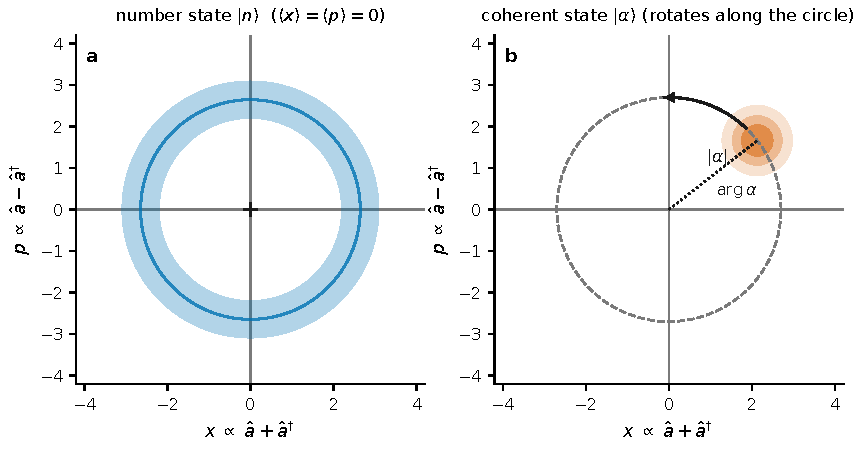
\includegraphics[width=0.92\linewidth]{figures/generated/edu_ch04/e04_phase_space_states.pdf}
\caption{相空间里两种极端量子态（横轴 \(x\propto\hat a+\hat a^\dagger\)，纵轴 \(p\propto\hat a-\hat a^\dagger\)）。左：数态 \(|n\rangle\) 的能量确定（环半径的平方固定），却把概率均匀地摊在整整一圈上，位置和动量的期望都为零、相位完全不定，像一枚模糊的圆环。右：相干态 \(|\alpha\rangle\) 凝成一小团紧凑光斑，钉在半径约 \(|\alpha|\)、方位角为 \(\arg\alpha\) 的圆周上，并沿圆周匀速旋转，复现出经典的正弦振动。}
\label{fig:e04-phase-space}
\end{figure}

这里我们只把定义 \eqref{eq:e04-coherent} 摆出来、给个直觉，具体展开——它的光子数服从泊松分布、它如何写成数态的叠加、它为什么是激光和恒星热光的自然出发点——留到第 \ref{chap:e06} 章。你只需记住一句话：数态是“能量最确定、相位最模糊”的极端，相干态是“相位最清晰、最像经典摆动”的对立极端，而它们用的是同一套 \(\hat a,\hat a^\dagger\)。

\section{本章要点}
\label{sec:e04-summary}

\begin{itemize}
  \item 谐振子的全部量子结构，只需要一条正则对易关系 \([\hat x,\hat p]=i\hbar\)。由它出发定义 \(\hat a,\hat a^\dagger\)（式 \eqref{eq:e04-adef}），逐项计算即得核心关系 \([\hat a,\hat a^\dagger]=1\)（式 \eqref{eq:e04-aacomm}），此后可以只在 \(\hat a,\hat a^\dagger\) 的代数里工作。
  \item 哈密顿量被改写成 \(\hat H=\hbar\omega(\hat n+\tfrac12)\)，其中数算符 \(\hat n=\hat a^\dagger\hat a\)。那个 \(+\tfrac12\) 是零点能 \(\tfrac12\hbar\omega\)，是测不准关系不允许振子绝对静止的直接后果。
  \item 用 \([\hat n,\hat a]=-\hat a\)、\([\hat n,\hat a^\dagger]=+\hat a^\dagger\) 证明 \(\hat a,\hat a^\dagger\) 逐级降/升本征值；用 \(\langle n|\hat a^\dagger\hat a|n\rangle=n\ge0\) 逼出本征值必为非负整数，阶梯在 \(\hat a|0\rangle=0\) 处封底。
  \item 归一化给出 \(\hat a|n\rangle=\sqrt{n}\,|n-1\rangle\)、\(\hat a^\dagger|n\rangle=\sqrt{n+1}\,|n+1\rangle\)，能谱是等间距梯子 \(E_n=\hbar\omega(n+\tfrac12)\)。相邻能级间隔 \(\hbar\omega\) 就是“一个光子”的能量。
  \item 数态是能量最确定、相位最模糊的态；相干态 \(|\alpha\rangle\)（\(\hat a|\alpha\rangle=\alpha|\alpha\rangle\)）则最接近经典振动，详见第 \ref{chap:e06} 章。
\end{itemize}

\paragraph{想一想。}
\begin{itemize}
  \item 如果把 \([\hat x,\hat p]=i\hbar\) 换成经典的 \([\hat x,\hat p]=0\)，重走一遍推导，你会发现 \([\hat a,\hat a^\dagger]\) 变成什么？能级还会离散吗？这说明离散能级到底是谁的功劳。
  \item 数态 \(|n\rangle\) 的位置期望值 \(\langle\hat x\rangle=0\)，但 \(\langle\hat x^2\rangle\) 却随 \(n\) 增大。试用式 \eqref{eq:e04-xp-in-a} 和式 \eqref{eq:e04-ladder-action} 算出 \(\langle n|\hat x^2|n\rangle\)，看看它是不是正比于 \((n+\tfrac12)\)——并解释这个结果和零点能的联系。
  \item 为什么说“吸收一个 \(\hbar\omega\) 的量子”对电磁场就是“多一个光子”？把谐振子的能量阶梯和光子数联系起来，用你自己的话讲一遍。
\end{itemize}
